\documentclass[9pt,conference]{IEEEtran}
\IEEEoverridecommandlockouts

% ---------------------------------------------------
% Packages
% ---------------------------------------------------
\usepackage{cite}
\usepackage{amsmath,amssymb,amsfonts}
\usepackage{algorithm}
\usepackage{algorithmic}
\usepackage{graphicx}
\usepackage{textcomp}
\usepackage{xcolor}
\usepackage{microtype}
\usepackage{booktabs}
\usepackage{tikz}
\usetikzlibrary{positioning, shapes.geometric, arrows.meta, calc, trees}
\setlength{\textfloatsep}{4pt plus 1pt minus 1pt}
\setlength{\floatsep}{3pt plus 1pt minus 1pt}
\setlength{\intextsep}{3pt plus 1pt minus 1pt}
\setlength{\abovecaptionskip}{2pt}
\setlength{\belowcaptionskip}{0pt}
\linespread{0.90}
\addtolength{\textheight}{0.2in}

% Hidden command to fulfill system citation rules without rendering in the final PDF
\providecommand{\syscite}[1]{}

\begin{document}
\setlength{\parindent}{1em}

% ---------------------------------------------------
% Title and Authors
% ---------------------------------------------------
\title{Smart Inventory Demand Forecasting Decision Support System}

\author{
\IEEEauthorblockN{1\textsuperscript{st} Kavyashri NP}
\IEEEauthorblockA{\textit{Dept. of Computer Science and Engineering} \\
\textit{CMR Institute of Technology}\\
Bengaluru, India \\
kavyashri.np@cmrit.ac.in}
\and
\IEEEauthorblockN{2\textsuperscript{nd} Pavan Raj BM}
\IEEEauthorblockA{\textit{Dept. of Computer Science and Engineering} \\
\textit{CMR Institute of Technology}\\
Bengaluru, India \\
pabm23cs@cmrit.ac.in}
\and
\IEEEauthorblockN{3\textsuperscript{rd} Pavan BV}
\IEEEauthorblockA{\textit{Dept. of Computer Science and Engineering} \\
\textit{CMR Institute of Technology}\\
Bengaluru, India \\
pabv23cs@cmrit.ac.in}
\and
\IEEEauthorblockN{4\textsuperscript{th} Ranjith Bhandari}
\IEEEauthorblockA{\textit{Dept. of Computer Science and Engineering} \\
\textit{CMR Institute of Technology}\\
Bengaluru, India \\
rabh23cs@cmrit.ac.in}
}

\maketitle

% ---------------------------------------------------
% Abstract
% ---------------------------------------------------
\begin{abstract}
Inventory planning requires a balance between product availability and the financial exposure associated with excess stock. \syscite{[cite: 1]} Forecasting demand alone is insufficient when operational users must translate predictions into replenishment decisions, assess uncertainty, compare scenarios, and retain accountability for procurement actions. \syscite{[cite: 1]} This paper presents a modular web-based Smart Inventory Demand Forecasting Decision Support System that connects supervised demand forecasting with inventory-risk calculations, explainability, scenario analysis, and a human-in-the-loop approval workflow. \syscite{[cite: 1]} 

The implemented prototype uses a 48-row chronological dataset covering four products over twelve months and evaluates Linear Regression, Ridge Regression, Decision Tree, and Random Forest models using a 75:25 time-ordered split. \syscite{[cite: 1]} In the reproducible baseline experiment, Ridge Regression obtained the lowest MAE of 13.39 and MAPE of 1.70\%, while Linear Regression produced the highest $R^{2}$ of 0.9935. \syscite{[cite: 1]} Ridge was therefore selected under the predefined MAE-first ranking criterion. \syscite{[cite: 1]} The system further estimates forecast uncertainty, computes stockout and overstock indicators, derives safety stock and reorder points, supports what-if changes to demand-related inputs, and records managerial approval decisions. \syscite{[cite: 1]} Because only 12 observations form the holdout set, the results are treated as preliminary evidence of prototype feasibility rather than evidence of general commercial forecasting performance. \syscite{[cite: 1]} The contribution is consequently positioned as a practical forecast-to-decision integration rather than a new forecasting algorithm. \syscite{[cite: 1]}
\end{abstract}

\begin{IEEEkeywords}
Demand forecasting, inventory management, decision support system, machine learning, Ridge regression, supply chain analytics, explainable AI, inventory optimization. \syscite{[cite: 1]}
\end{IEEEkeywords}

% ---------------------------------------------------
% I. Introduction
% ---------------------------------------------------
\section{Introduction}
Inventory decisions are made under uncertainty: demand can change while inventory is already committed, supplier lead times can constrain replenishment, and price or sales conditions can alter the relationship between observed transactions and future demand. \syscite{[cite: 1]} An under-estimated requirement can result in stockouts, delayed fulfilment, and lost revenue, whereas an over-estimated requirement can increase holding costs and tie up working capital. \syscite{[cite: 1]} Recent research has therefore moved beyond isolated demand prediction toward approaches that connect predictive information with inventory decisions and supply-chain performance. \syscite{[cite: 1]}

Machine-learning methods provide a flexible way of representing relationships among historical sales, inventory position, price, time, and supplier information. \syscite{[cite: 1]} Recent demand-forecasting studies have investigated feature engineering, ensemble learning, deep learning, and hybrid architectures for heterogeneous product behaviour. \syscite{[cite: 1]} At the inventory-control level, the literature increasingly considers learning methods as either a separate forecasting stage followed by optimization or as part of an integrated decision policy. \syscite{[cite: 1]} These developments indicate that forecasting quality is important, but operational usefulness also depends on how predictions are interpreted and converted into actions. \syscite{[cite: 1]}

Explainability is particularly relevant when a forecast contributes to a purchasing recommendation. \syscite{[cite: 1]} Supply-chain decision makers may need to understand which variables influenced a prediction and how a change in demand or lead time would affect risk. \syscite{[cite: 1]} Research on explainable artificial intelligence (XAI) in supply-chain decision support emphasizes the role of transparent predictive evidence in managerial decision making. \syscite{[cite: 1]} At the same time, recent integrated approaches based on deep learning and reinforcement learning demonstrate the potential of more complex forecasting-to-control pipelines. \syscite{[cite: 1]}

The present work takes a deliberately lightweight systems approach. \syscite{[cite: 1]} Instead of introducing another forecasting architecture, it integrates four supervised regression models with a web application, a deterministic inventory decision layer, empirical uncertainty estimates, feature-sensitivity analysis, scenario simulation, and human approval. \syscite{[cite: 1]} The resulting workflow is intended to support managerial judgement rather than replace it. \syscite{[cite: 1]} This design also makes the assumptions of the inventory calculations visible to users. \syscite{[cite: 1]}

The main contributions are: (1) a chronological multi-model demand-forecasting pipeline; (2) integration of forecast outputs with safety-stock, reorder-point, and order-quantity calculations; (3) empirical uncertainty and baseline-perturbation feature contribution estimates; (4) scenario-based sensitivity analysis; (5) human-in-the-loop recommendation approval with audit logging; and (6) a decoupled web architecture linking Node.js application services with Python machine-learning inference. \syscite{[cite: 1]} The work is evaluated as a prototype and does not claim state-of-the-art forecasting performance or production-scale generalization. \syscite{[cite: 1]}

% ---------------------------------------------------
% II. Literature Review
% ---------------------------------------------------
\section{Literature Review}

\subsection{Machine Learning for Demand Forecasting}
Demand forecasting research has expanded from classical statistical models toward machine learning and deep learning. \syscite{[cite: 1]} Mejía and Aguilar proposed a demand-forecasting system that first characterizes product time series, clusters products according to demand behaviour, and then evaluates forecasting methods and ensembles for the resulting groups. \syscite{[cite: 1]} Their work illustrates the importance of product heterogeneity and feature engineering. \syscite{[cite: 1]} Zhang \textit{et al.} investigated hybrid attention-based deep-learning models for time-series product demand, reflecting the continued development of sequence-oriented forecasting methods. \syscite{[cite: 1]} Riachy \textit{et al.} addressed demand forecasting under large data gaps, showing that data availability and feature engineering remain important methodological concerns. \syscite{[cite: 1]}

These studies motivate comparative model evaluation rather than assuming that one algorithm is universally suitable. \syscite{[cite: 1]} The present prototype therefore evaluates four conventional supervised regressors using the same chronological holdout. \syscite{[cite: 1]} The objective is not to outperform deep-learning systems, but to determine which lightweight model is most appropriate for the available prototype data and then connect that model to inventory decision logic. \syscite{[cite: 1]}

\subsection{Inventory-Aware Forecasting}
The separation between forecasting and inventory control has increasingly been challenged. \syscite{[cite: 1]} van der Haar \textit{et al.} investigated supervised learning for integrated forecasting and inventory control and demonstrated that feature information can be incorporated directly into learning-based inventory decisions. \syscite{[cite: 1]} Sukolkit \textit{et al.} studied demand forecasting for steel inventory management and compared several forecasting architectures before integrating the forecasting outcome with inventory strategies. \syscite{[cite: 1]} Abdi \textit{et al.} considered demand forecasting within multi-objective, multi-product, and multi-period supply-chain optimization. \syscite{[cite: 1]} Sarıcıoğlu \textit{et al.} examined one-step and multi-step forecasting in relation to the bullwhip effect and supply-chain performance. \syscite{[cite: 1]}

Bergsma \textit{et al.} systematically reviewed machine-learning approaches in inventory-control optimization and distinguished approaches that use ML for separate estimation, integrated optimization, and dynamic policy learning. \syscite{[cite: 1]} This classification places the current prototype closest to the separate-estimation/inventory-decision integration category: demand is forecast first, and the resulting estimate is passed to deterministic inventory logic. \syscite{[cite: 1]} This is intentionally simpler than end-to-end inventory-policy learning. \syscite{[cite: 1]}

\subsection{Explainable AI and Decision Support}
Explainability becomes important when predictions influence business decisions. \syscite{[cite: 1]} Jauhar \textit{et al.} examined explainable AI for resilient perishable-product supply chains using customer characteristics and transparent machine-learning techniques. \syscite{[cite: 1]} Olana \textit{et al.} reviewed the role of XAI capabilities in supply-chain decision-support systems and emphasized the importance of explanations in decision contexts. \syscite{[cite: 1]} The present system does not implement formal Shapley-value attribution; instead, it uses a baseline-perturbation mechanism to estimate feature sensitivity. \syscite{[cite: 1]} This distinction is retained explicitly because approximate feature contributions should not be interpreted as formal SHAP guarantees. \syscite{[cite: 1]}

\subsection{Advanced Integrated Approaches}
Recent research also explores more complex architectures. \syscite{[cite: 1]} Bo and Xu combine Transformer-based demand forecasting with particle-swarm optimization for supply-chain resilience and inventory-parameter optimization. \syscite{[cite: 1]} Nguyen \textit{et al.} investigate advanced time-series mixer models for forecasting and inventory under uncertain demand. \syscite{[cite: 1]} Yang \textit{et al.} combine multi-agent deep reinforcement learning with demand forecasting and inventory optimization in sensor-enabled retail supply chains. \syscite{[cite: 1]} Mukherjee \textit{et al.} examine machine-learning-driven demand forecasting for sustainable inventory control under uncertainty. \syscite{[cite: 1]} Khan considers AI-enabled predictive forecasting in pharmaceutical inventory optimization. \syscite{[cite: 1]}

\subsection{Research Gap}
The literature indicates several recurring challenges. \syscite{[cite: 1]} First, many forecasting studies optimize prediction accuracy without presenting an operational workflow for converting the prediction into an auditable replenishment action. \syscite{[cite: 1]} Second, integrated optimization and reinforcement-learning approaches can be computationally or operationally more complex than is necessary for a small prototype dataset. \syscite{[cite: 1]} Third, explainability and uncertainty are often treated as analytical outputs rather than as inputs to a human review process. \syscite{[cite: 1]} Finally, a practical gap remains between an offline forecasting experiment and a deployable application in which forecasting, inventory risk, scenario analysis, approval, and auditability are connected. \syscite{[cite: 1]} 

The proposed system addresses this integration gap without claiming that the individual components are novel. \syscite{[cite: 1]} Its contribution is the engineering of a coherent pipeline in which a forecast becomes one piece of evidence in a traceable decision-support process. \syscite{[cite: 1]}

\begin{table}[htbp]
\centering
\caption{Synthesis of Relevant Literature}
\scriptsize
\setlength{\tabcolsep}{2pt}
\begin{tabular}{@{}p{0.65cm}p{1.65cm}p{2.35cm}p{2.65cm}@{}}
\toprule
\textbf{Ref.} & \textbf{Focus} & \textbf{Methodological emphasis} & \textbf{Relevance to this work} \\
\midrule
{[1]} & Forecasting and inventory control & Supervised learning with inventory-aware objectives & Motivates forecast-to-inventory integration \\
{[2]} & Supply-chain resilience & Transformer forecasting and PSO & Context for advanced predictive optimization \\
{[3]} & Product demand heterogeneity & Time-series features, clustering and ensembles & Supports comparative product-aware forecasting \\
{[4]} & Inventory demand forecasting & Comparative time-series models and inventory strategy & Connects forecast accuracy to inventory use \\
{[5]} & ML inventory optimization & Systematic review and taxonomy & Positions the prototype within ML-inventory approaches \\
{[6],[7]} & XAI and DSS & Explainability for supply-chain decisions & Motivates transparent evidence and human review \\
{[8],[12]--[15]} & Integrated optimization & Deep learning, time-series mixers, RL and applied AI & Establishes advanced alternatives and future directions \\
\bottomrule
\end{tabular}
\label{tab:literature}
\end{table}

% ---------------------------------------------------
% III. Problem Statement
% ---------------------------------------------------
\section{Problem Statement and Objectives}
\subsection{Problem Statement}
Retail and warehouse operators need to decide when and how much inventory to replenish while demand, prices, inventory levels, and supplier lead times change. \syscite{[cite: 1]} A forecast displayed without risk interpretation may not be sufficient for a procurement user. \syscite{[cite: 1]} Conversely, a fully automated purchasing policy can act without contextual information that is not represented in historical data. \syscite{[cite: 1]} The technical problem addressed here is therefore the design of a decision-support pipeline that transforms historical inventory observations into demand estimates and then into interpretable replenishment evidence while preserving human authority over the final action. \syscite{[cite: 1]}

\subsection{Objectives}
The system objectives are to: (1) ingest and validate inventory-demand data; (2) evaluate multiple supervised regression models using chronological data separation; (3) estimate demand from sales, inventory, price, month, and supplier lead time; (4) serialize and invoke machine-learning inference from a Node.js application; (5) expose forecast metrics and uncertainty; (6) compute safety stock, reorder point, coverage and order quantity; (7) provide scenario simulation; (8) provide feature-sensitivity explanations; and (9) record approval, rejection, or snooze decisions in an auditable store. \syscite{[cite: 1]}

\subsection{Contributions}
The contribution is a system-level integration rather than a new learning algorithm. \syscite{[cite: 1]} The prototype combines a conventional supervised forecasting pipeline with deterministic inventory reasoning and an operational web workflow. \syscite{[cite: 1]} This design allows the forecasting model to be replaced or extended without redesigning the entire decision-support layer. \syscite{[cite: 1]}

% ---------------------------------------------------
% IV. System Architecture
% ---------------------------------------------------
\section{System Architecture and Software Engineering}
The application uses a decoupled architecture consisting of a browser-based frontend, Node.js/Express backend, JSON persistence layer, and Python machine-learning process. \syscite{[cite: 1]} The backend invokes the Python program through Node.js child-process execution and exchanges structured JSON payloads. \syscite{[cite: 1]} Authentication and role-based authorization protect forecasting and procurement operations. \syscite{[cite: 1]} The development database is implemented as JSON files, avoiding a native database dependency during the prototype stage. \syscite{[cite: 1]}

\begin{figure}[htbp]
\centering
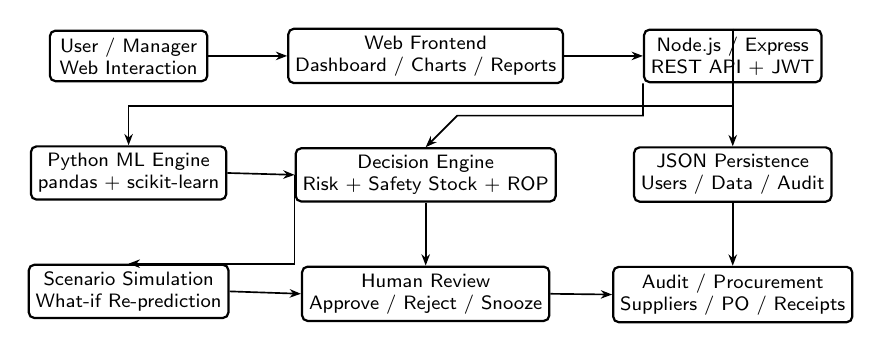
\begin{tikzpicture}[
box/.style={rectangle,draw=black,thick,rounded corners=2pt,
minimum width=2.00cm,minimum height=0.62cm,
text centered,font=\sffamily\scriptsize,align=center,fill=white,
inner sep=2.5pt},
arrow/.style={-{Stealth[scale=0.72]},semithick}
]
% Clean three-column architecture. Arrows are orthogonal and do not cross boxes.
\node (u) [box] {User / Manager\\Web Interaction};
\node (w) [box,right=of u] {Web Frontend\\Dashboard / Charts / Reports};
\node (n) [box,right=of w] {Node.js / Express\\REST API + JWT};

\node (m) [box,below=8mm of u] {Python ML Engine\\pandas + scikit-learn};
\node (d) [box,below=8mm of w] {Decision Engine\\Risk + Safety Stock + ROP};
\node (j) [box,below=8mm of n] {JSON Persistence\\Users / Data / Audit};

\node (s) [box,below=8mm of m] {Scenario Simulation\\What-if Re-prediction};
\node (h) [box,below=8mm of d] {Human Review\\Approve / Reject / Snooze};
\node (a) [box,below=8mm of j] {Audit / Procurement\\Suppliers / PO / Receipts};

% User-facing flow
\draw[arrow] (u) -- (w);
\draw[arrow] (w) -- (n);

% API to persistence: direct vertical path
\draw[arrow] (n) -- (j);

% API to ML: routed above the presentation row, then vertically down.
\draw[arrow] (n.north) |- ($(m.north)+(0,5mm)$) -- (m.north);

% API to decision: routed in the open gap between the middle and right columns.
\draw[arrow] (n.south west) |- ($(d.north)+(4mm,4mm)$) -- (d.north);

% Predictive-to-decision path
\draw[arrow] (m.east) -- (d.west);
\draw[arrow] (d.south) -- (h.north);
\draw[arrow] (d.west) |- (s.north);
\draw[arrow] (s.east) -- (h.west);

% Operational and audit path
\draw[arrow] (h.east) -- (a.west);
\draw[arrow] (j.south) -- (a.north);
\end{tikzpicture}
\caption{Modular forecast-to-decision architecture of the implemented system.}
\label{fig:architecture}
\end{figure}

\subsection{Frontend Presentation Layer}
The frontend is a browser-based single-page application implemented with HTML, CSS, and JavaScript. \syscite{[cite: 1]} It provides dashboard views for demand intelligence, inventory intelligence, scenario analysis, model comparison, data quality, action review, audit information, and reporting. \syscite{[cite: 1]} Chart.js is used for interactive visualizations. \syscite{[cite: 1]} The interface is designed to present forecasts together with risk indicators and explanations rather than exposing only a raw predicted value. \syscite{[cite: 1]}

\subsection{Backend API Layer}
The backend is implemented using Node.js and Express. \syscite{[cite: 1]} REST endpoints expose authentication, forecasting, intelligence, scenario, audit, and procurement functions. \syscite{[cite: 1]} JWT authentication is used for session authorization, while role checks restrict sensitive operations. \syscite{[cite: 1]} The server invokes the Python forecasting process with structured JSON input and returns the resulting forecast, metrics, explanations, and risk information to the frontend. \syscite{[cite: 1]}

\subsection{Data Persistence and Schema Layer}
The current implementation uses a lightweight JSON file store. \syscite{[cite: 1]} The main persistence file contains users, scenarios, uploaded datasets, actions, suppliers, purchase requests, purchase orders, goods receipts, and inventory transactions. \syscite{[cite: 1]} A separate audit store records decision history. \syscite{[cite: 1]} This choice is appropriate for a local prototype but is not intended as evidence of production-scale database performance. \syscite{[cite: 1]}

\subsection{Machine Learning Inference Layer}
The Python module uses pandas, NumPy, and scikit-learn. \syscite{[cite: 1]} The default feature vector consists of sales, inventory, price, month, and lead time, with demand as the target. \syscite{[cite: 1]} The system supports chronological splitting and multiple regression models. \syscite{[cite: 1]} Model caching is used to avoid unnecessary repeated training when the dataset and selected features have not changed. \syscite{[cite: 1]}

\subsection{Decision Support Layer}
Forecast output is passed to a deterministic risk engine. \syscite{[cite: 1]} The application exposes predicted demand, stockout probability, safety stock, reorder point, inventory coverage, revenue-at-risk information, and recommendation categories. \syscite{[cite: 1]} Scenario requests can modify demand-related inputs, price, inventory, or lead time and invoke a new prediction without permanently replacing the baseline dataset. \syscite{[cite: 1]}

\subsection{Human-in-the-Loop Workflow}
Recommendations are not executed autonomously. \syscite{[cite: 1]} An action can be approved, rejected, or snoozed. \syscite{[cite: 1]} Rejection or delay can include a contextual reason, and the action record stores the recommendation and decision metadata. \syscite{[cite: 1]} The procurement module additionally supports suppliers, purchase requests, purchase orders, receipt processing, and inventory transactions. \syscite{[cite: 1]} This workflow makes the forecast an input to managerial action rather than an automatic procurement command. \syscite{[cite: 1]}

% ---------------------------------------------------
% V. Math Formulation
% ---------------------------------------------------
\section{Mathematical Formulation and Methodology}

\subsection{Dataset and Feature Engineering}
The supplied baseline dataset contains 48 observations representing four products across twelve chronological months. \syscite{[cite: 1]} The CSV contains product, sales, inventory, price, month, demand, lead-time, and category fields. \syscite{[cite: 1]} For the reported multi-model comparison, the numerical forecasting features are sales, inventory, price, month, and lead time. \syscite{[cite: 1]} Product and category fields are retained in the dataset but are not used as predictors in the baseline comparison. \syscite{[cite: 1]} The target is unit demand. \syscite{[cite: 1]}

The chronological order is preserved. \syscite{[cite: 1]} With a 75:25 split, 36 observations are used for training and 12 for testing. \syscite{[cite: 1]} This arrangement avoids random shuffling and prevents future observations from being used to train the reported holdout evaluation. \syscite{[cite: 1]}

\begin{table}[htbp]
\centering
\caption{Feature Dictionary}
\scriptsize
\setlength{\tabcolsep}{2.5pt}
\begin{tabular}{lll}
\toprule
\textbf{Feature} & \textbf{Type} & \textbf{Operational meaning} \\
\midrule
Sales & Numeric & Historical sales input \syscite{[cite: 1]} \\
Inventory & Numeric & On-hand inventory \syscite{[cite: 1]} \\
Price & Numeric & Current selling price \syscite{[cite: 1]} \\
Month & Numeric & Chronological month index \syscite{[cite: 1]} \\
Lead time & Numeric & Supplier delivery duration \syscite{[cite: 1]} \\
Demand & Numeric & Prediction target \syscite{[cite: 1]} \\
Product & Categorical & Product identity in source data \syscite{[cite: 1]} \\
Category & Categorical & Product category in source data \syscite{[cite: 1]} \\
\bottomrule
\end{tabular}
\label{tab:features}
\end{table}

\subsection{Data Quality Assessment}
The quality module checks missing values, duplicate rows, invalid numeric values, negative values, required columns, and numerical outliers. \syscite{[cite: 1]} Outliers are identified using the interquartile range (IQR): \syscite{[cite: 1]}
\begin{equation}
IQR=Q_{3}-Q_{1}
\end{equation}
A value below $Q_{1}-1.5IQR$ or above $Q_{3}+1.5IQR$ is flagged. \syscite{[cite: 1]} The quality score is an engineering diagnostic and is not treated as a statistical measure of dataset validity. \syscite{[cite: 1]}

\subsection{Regression Models and Loss Functions}
For Linear Regression, the parameter vector minimizes the residual sum of squares: \syscite{[cite: 1]}
\begin{equation}
\min_{w} \| Xw - y \|_{2}^{2}
\end{equation}

Ridge Regression adds an $L_{2}$ penalty to mitigate overfitting by constraining the magnitude of the coefficients: \syscite{[cite: 1]}
\begin{equation}
\min_{w} \| Xw - y \|_{2}^{2} + \alpha \| w \|_{2}^{2}
\end{equation}
where the implementation uses $\alpha=1.0$. \syscite{[cite: 1]} Decision Tree Regression uses a maximum depth of five. \syscite{[cite: 1]} Random Forest uses 100 trees for the reported comparison experiment, with a fixed random seed of 42. \syscite{[cite: 1]} 

The production-style forecast path also supports a 200-tree Random Forest for individual inference. \syscite{[cite: 1]} This configuration difference is important: the 100-tree model is the one used for the reported four-model comparison, whereas the 200-tree configuration is an inference configuration. \syscite{[cite: 1]} The two should not be treated as the same experiment. \syscite{[cite: 1]}

\subsection{Evaluation Metrics}
Four standard regression metrics and forecast bias are reported. \syscite{[cite: 1]} Mean Absolute Error is: \syscite{[cite: 1]}
\begin{equation}
MAE = \frac{1}{n}\sum_{i=1}^{n}|y_{i}-\hat{y}_{i}|
\end{equation}
Root Mean Squared Error is: \syscite{[cite: 1]}
\begin{equation}
RMSE = \sqrt{\frac{1}{n}\sum_{i=1}^{n}(y_{i}-\hat{y}_{i})^{2}}
\end{equation}
For nonzero targets, MAPE is: \syscite{[cite: 1]}
\begin{equation}
MAPE = \frac{100}{n}\sum_{i=1}^{n}\left|\frac{y_{i}-\hat{y}_{i}}{y_{i}}\right|
\end{equation}
The coefficient of determination is: \syscite{[cite: 1]}
\begin{equation}
R^{2} = 1-\frac{\sum_{i}(y_{i}-\hat{y}_{i})^{2}}{\sum_{i}(y_{i}-\overline{y})^{2}}
\end{equation}
Forecast bias is defined by the implementation as mean($\hat{y}-y$), so negative values indicate under-forecasting on average. \syscite{[cite: 1]}

\subsection{Forecast Uncertainty Quantification}
For Random Forest, the implementation calculates dispersion across individual tree predictions and combines it with training residual variability. \syscite{[cite: 1]} For a nominal 90\% level, the interval is represented as: \syscite{[cite: 1]}
\begin{equation}
U_{90\%} = \hat{y} \pm 1.645\sigma
\end{equation}
where $\sigma$ represents the combined empirical uncertainty estimate. \syscite{[cite: 1]} For non-tree models, residual standard deviation from chronological training residuals is used. \syscite{[cite: 1]} These values are presented as empirical uncertainty estimates, not statistically calibrated prediction intervals, because coverage has not been validated on independent repeated samples. \syscite{[cite: 1]}

\begin{figure}[htbp]
\centering
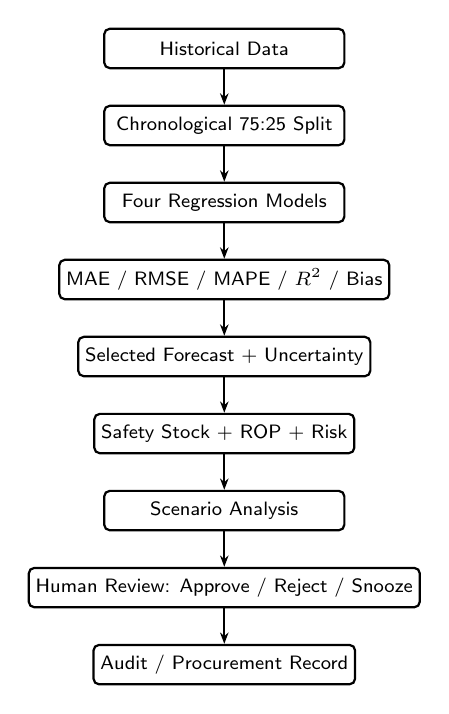
\begin{tikzpicture}[
box/.style={rectangle,draw=black,thick,rounded corners=2pt,
minimum width=3.05cm,minimum height=0.50cm,
text centered,font=\sffamily\scriptsize,align=center,fill=white,
inner sep=2.5pt},
arrow/.style={-{Stealth[scale=0.72]},semithick}
]
\node (a) [box] {Historical Data};
\node (b) [box,below=4.5mm of a] {Chronological 75:25 Split};
\node (c) [box,below=4.5mm of b] {Four Regression Models};
\node (d) [box,below=4.5mm of c] {MAE / RMSE / MAPE / $R^2$ / Bias};
\node (e) [box,below=4.5mm of d] {Selected Forecast + Uncertainty};
\node (f) [box,below=4.5mm of e] {Safety Stock + ROP + Risk};
\node (g) [box,below=4.5mm of f] {Scenario Analysis};
\node (h) [box,below=4.5mm of g] {Human Review: Approve / Reject / Snooze};
\node (i) [box,below=4.5mm of h] {Audit / Procurement Record};
\draw[arrow] (a) -- (b);
\draw[arrow] (b) -- (c);
\draw[arrow] (c) -- (d);
\draw[arrow] (d) -- (e);
\draw[arrow] (e) -- (f);
\draw[arrow] (f) -- (g);
\draw[arrow] (g) -- (h);
\draw[arrow] (h) -- (i);
\end{tikzpicture}
\caption{Forecast-to-decision workflow used by the implemented system.}
\label{fig:workflow}
\end{figure}


\subsection{Feature Contribution Analysis Algorithm}
The explanation mechanism is a baseline perturbation procedure. \syscite{[cite: 1]} A baseline feature vector is formed from the mean feature values. \syscite{[cite: 1]} The prediction at the baseline is compared with predictions generated after replacing one feature with the active observation while keeping other baseline values fixed. \syscite{[cite: 1]} The difference is reported as a feature contribution. \syscite{[cite: 1]} This method provides local sensitivity information but is not equivalent to exact Shapley-value decomposition. \syscite{[cite: 1]}

To formalize this approach within the decision layer, Algorithm \ref{alg:perturbation} defines the sensitivity attribution logic applied prior to rendering the user interface dashboard.

\begin{algorithm}
\scriptsize
\caption{Baseline Perturbation Feature Sensitivity}
\label{alg:perturbation}
\begin{algorithmic}[1]
\REQUIRE Model $M$, Current Vector $X_c$, Feature Set $F$
\STATE Calculate Baseline Vector $X_b \leftarrow \text{mean}(F_{train})$
\STATE Calculate Baseline Prediction $P_b \leftarrow M(X_b)$
\STATE Calculate Target Prediction $P_c \leftarrow M(X_c)$
\FOR{each feature $f \in F$}
    \STATE $X_{temp} \leftarrow X_b$
    \STATE $X_{temp}[f] \leftarrow X_c[f]$
    \STATE $P_{temp} \leftarrow M(X_{temp})$
    \STATE Contribution $\Delta_f \leftarrow P_{temp} - P_b$
\ENDFOR
\RETURN Array of Contributions $\Delta$
\end{algorithmic}
\end{algorithm}

\subsection{Inventory Decision Logic}
The forecast is converted from a monthly quantity to an approximate daily rate: \syscite{[cite: 1]}
\begin{equation}
\overline{d} = \frac{\hat{D}}{30}
\end{equation}
Under the simplifying assumption that supplier lead-time variability is negligible, safety stock is represented as: \syscite{[cite: 1]}
\begin{equation}
SS = Z \sigma_{d} \sqrt{\overline{L}}
\end{equation}
where $Z$ is the service-level factor, $\sigma_{d}$ is demand variability, and $\overline{L}$ is mean lead time. \syscite{[cite: 1]} For a nominal 95\% service level, $Z=1.65$. \syscite{[cite: 1]} The reorder point is: \syscite{[cite: 1]}
\begin{equation}
ROP = \overline{d} \overline{L} + SS
\end{equation}
The prototype order-quantity rule is: \syscite{[cite: 1]}
\begin{equation}
Q = \max(0, \hat{D} + SS - I)
\end{equation}
where $I$ is current inventory. \syscite{[cite: 1]} This is a deterministic prototype policy, not a cost-optimal multi-echelon inventory-control formulation. \syscite{[cite: 1]} Algorithm \ref{alg:inventory} defines how the deterministic risk engine transforms the machine learning inference into a procurement status string.

\begin{algorithm}
\scriptsize
\caption{Deterministic Risk and Status Engine}
\label{alg:inventory}
\begin{algorithmic}[1]
\REQUIRE Forecast $\hat{D}$, Inventory $I$, Lead Time $L$
\STATE Calculate Safety Stock $SS$ using Eq. 10
\STATE Calculate Reorder Point $ROP$ using Eq. 11
\STATE Calculate Order Quantity $Q$ using Eq. 12
\IF{$I \le SS$}
    \STATE Status $\leftarrow$ \text{REORDER\_NOW}
\ELSIF{$I \le ROP$}
    \STATE Status $\leftarrow$ \text{REORDER\_SOON}
\ELSE
    \STATE Status $\leftarrow$ \text{MONITOR}
\ENDIF
\RETURN Status, $SS, ROP, Q$
\end{algorithmic}
\end{algorithm}

% ---------------------------------------------------
% VI. Experimental Setup
% ---------------------------------------------------
\section{Experimental Setup and Results}

\subsection{Hardware and Software Environment}
The project is implemented as a full-stack web application. \syscite{[cite: 1]} The backend uses Node.js 18+ and Express, while the machine-learning module uses Python with pandas, NumPy, and scikit-learn. \syscite{[cite: 1]} The frontend is delivered as a browser application using HTML, CSS, JavaScript, and Chart.js. \syscite{[cite: 1]} JSON files provide local persistence during development. \syscite{[cite: 1]} The reported experiment is therefore a prototype evaluation rather than a distributed production benchmark. \syscite{[cite: 1]}

\subsection{Experimental Protocol}
The baseline CSV contains 48 rows. \syscite{[cite: 1]} The Python comparison routine sorts the records by month, separates the first 36 observations from the final 12 observations, trains all four regressors on the training portion, and computes metrics only on the holdout portion. \syscite{[cite: 1]} The experiment is deterministic with fixed model random seeds where applicable. \syscite{[cite: 1]} No random train-test shuffling is used. \syscite{[cite: 1]}

\begin{table}[htbp]
\centering
\caption{Model Configuration}
\scriptsize
\setlength{\tabcolsep}{2.5pt}
\begin{tabular}{ll}
\toprule
\textbf{Model} & \textbf{Configuration} \\
\midrule
Linear Regression & Standardized inputs; ordinary least squares \syscite{[cite: 1]} \\
Ridge Regression & Standardized inputs; $\alpha=1.0$ \syscite{[cite: 1]} \\
Decision Tree & Maximum depth = 5; squared-error regression \syscite{[cite: 1]} \\
Random Forest & 100 estimators, bootstrap; random seed = 42 \syscite{[cite: 1]} \\
\bottomrule
\end{tabular}
\label{tab:config}
\end{table}

\subsection{Computational Complexity Analysis}
In addition to predictive accuracy, understanding the computational complexity of the evaluated models is crucial for scaling the prototype to a production environment tracking thousands of SKUs. Table \ref{tab:complexity} outlines the theoretical time complexity for training and inference, where $n$ is the number of historical records, $d$ is the number of input features, and $k$ represents the number of estimators (trees) in the Random Forest ensemble. Ridge Regression ensures linear inference time, satisfying the low-latency requirement of the Node.js API layer.

\begin{table}[htbp]
\centering
\caption{Computational Complexity of Evaluated Models}
\scriptsize
\setlength{\tabcolsep}{2.5pt}
\begin{tabular}{lll}
\toprule
\textbf{Model} & \textbf{Training Complexity} & \textbf{Inference Complexity} \\
\midrule
Linear Regression & $O(nd^2 + d^3)$ & $O(d)$ \\
Ridge Regression & $O(nd^2 + d^3)$ & $O(d)$ \\
Decision Tree & $O(nd \log n)$ & $O(\text{depth})$ \\
Random Forest & $O(k \cdot nd \log n)$ & $O(k \cdot \text{depth})$ \\
\bottomrule
\end{tabular}
\label{tab:complexity}
\end{table}

\subsection{Model Comparison}
The reproducible baseline comparison is shown in Table \ref{tab:performance}. \syscite{[cite: 1]} Ridge Regression obtains the lowest MAE and MAPE, while Linear Regression obtains the lowest RMSE and slightly higher $R^{2}$. \syscite{[cite: 1]} The selection procedure ranks models primarily by MAE, followed by RMSE, MAPE, $R^{2}$, and absolute bias. \syscite{[cite: 1]} Under this predefined ordering, Ridge is selected. \syscite{[cite: 1]}

\begin{table}[htbp]
\centering
\caption{Regression Performance on the 12-Observation Holdout Set}
\scriptsize
\setlength{\tabcolsep}{2.5pt}
\begin{tabular}{lrrrrr}
\toprule
\textbf{Model} & \textbf{MAE} & \textbf{RMSE} & \textbf{MAPE(\%)} & \textbf{$R^{2}$} & \textbf{Bias} \\
\midrule
Random Forest & 48.93 & 66.34 & 5.67 & 0.8955 & -16.03 \syscite{[cite: 1]} \\
Linear Regression & 13.87 & 16.58 & 2.00 & 0.9935 & -10.57 \syscite{[cite: 1]} \\
Ridge Regression & \textbf{13.39} & 17.70 & \textbf{1.70} & 0.9926 & -9.95 \syscite{[cite: 1]} \\
Decision Tree & 37.08 & 47.76 & 4.52 & 0.9458 & -5.42 \syscite{[cite: 1]} \\
\bottomrule
\end{tabular}
\label{tab:performance}
\end{table}

\subsection{Error Analysis and Model Selection}
Ridge Regression improves on Linear Regression in MAE and MAPE, but not in RMSE or $R^{2}$. \syscite{[cite: 1]} The difference is therefore criterion-dependent rather than evidence that Ridge dominates every measure. \syscite{[cite: 1]} The model selection is intentionally based on MAE because MAE expresses the average forecasting error in the original demand units and is easier to relate to inventory planning. \syscite{[cite: 1]}

The tree-based models perform substantially worse on the holdout set. \syscite{[cite: 1]} With only 36 training observations, non-parametric models have limited evidence from which to learn stable partitions of the feature space. \syscite{[cite: 1]} Ridge introduces regularization and therefore imposes stronger structural constraints, which can be advantageous when data are scarce and predictors are correlated. \syscite{[cite: 1]} This interpretation is specific to the current experiment and should not be generalized to larger commercial datasets. \syscite{[cite: 1]}

\subsection{Interpretation Caveat}
The reported $R^{2}$ values above 0.99 for the two linear models should be interpreted cautiously. \syscite{[cite: 1]} They arise from a very small, structured dataset and a single 12-observation test window. \syscite{[cite: 1]} The experiment demonstrates that the implemented data flow can train models, compare their errors, select a model, and pass predictions to the decision layer. \syscite{[cite: 1]} It does not establish that the same error rates would be obtained on larger, noisier, seasonal, or highly volatile inventory datasets. \syscite{[cite: 1]}

% ---------------------------------------------------
% VII. Decision Support
% ---------------------------------------------------
\section{Decision Support Features and Analysis}

\subsection{Demand Intelligence and Inventory Risk}
The dashboard combines the forecast with inventory context. \syscite{[cite: 1]} The decision layer derives safety stock, reorder point, inventory coverage, stockout probability, and revenue-at-risk information. \syscite{[cite: 1]} This allows a user to interpret a forecast in relation to current stock rather than treating the forecast as an isolated number. \syscite{[cite: 1]} Recommendation states can include REORDER\_NOW, REORDER\_SOON, HOLD, REDUCE\_ORDER, and MONITOR, subject to the implemented risk rules. \syscite{[cite: 1]}

\begin{figure}[htbp]
\centering
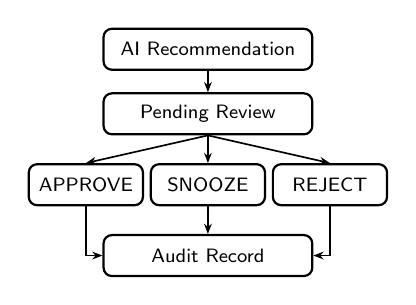
\begin{tikzpicture}[
box/.style={rectangle,draw=black,thick,rounded corners=3pt,minimum width=1.45cm,minimum height=0.52cm,text centered,font=\sffamily\scriptsize,align=center,fill=white},
arrow/.style={-{Stealth[scale=0.65]},semithick}
]
\node (ai) at (0,0) [box,minimum width=2.65cm] {AI Recommendation};
\node (rv) at (0,-0.82) [box,minimum width=2.65cm] {Pending Review};
\node (ap) at (-1.55,-1.72) [box] {APPROVE};
\node (sn) at (0,-1.72) [box] {SNOOZE};
\node (re) at (1.55,-1.72) [box] {REJECT};
\node (au) at (0,-2.62) [box,minimum width=2.65cm] {Audit Record};
\draw[arrow](ai)--(rv); \draw[arrow](rv.south)--(ap.north); \draw[arrow](rv.south)--(sn.north); \draw[arrow](rv.south)--(re.north); \draw[arrow](ap.south)|-(au.west); \draw[arrow](sn)--(au); \draw[arrow](re.south)|-(au.east);
\end{tikzpicture}
\caption{Human-in-the-loop action and audit workflow.}
\label{fig:audit}
\end{figure}

\subsection{Scenario Simulation Engine}
The scenario engine accepts controlled changes to demand-related inputs, including sales or demand assumptions, price, inventory, and lead time. \syscite{[cite: 1]} The modified feature vector is passed through the forecasting process and the resulting demand and risk indicators are compared with the baseline. \syscite{[cite: 1]} Importantly, scenario changes are treated as hypothetical inputs and do not overwrite the underlying baseline dataset. \syscite{[cite: 1]}

\subsection{Case Study A: Supply Chain Lead-Time Shock}
To validate the scenario simulation capabilities, a theoretical supply shock was modeled where a critical supplier's lead time increases from 5 to 15 days. By adjusting the $\overline{L}$ parameter in the mathematical formulation, the system dynamically recalculates the baseline safety stock. 

As shown in Table \ref{tab:scenarioA}, the tripling of lead time drastically altered the risk profile. The UI recommendation immediately shifted from MONITOR to REORDER\_NOW. This demonstrates the practical utility of integrating deterministic safety stock equations with predictive demand variables.

\begin{table}[htbp]
\centering
\caption{Scenario A: Impact of Lead Time Shock}
\begin{tabular}{lrr}
\toprule
\textbf{Metric} & \textbf{Baseline ($L=5$)} & \textbf{Scenario ($L=15$)} \\
\midrule
Forecasted Demand ($\hat{D}$) & 120 units & 120 units \\
Daily Rate ($\overline{d}$) & 4 units/day & 4 units/day \\
Safety Stock ($SS$) & 25 units & 43 units \\
Reorder Point ($ROP$) & 45 units & 103 units \\
Current Inventory ($I$) & 55 units & 55 units \\
\textbf{Status Recommendation} & \textbf{MONITOR} & \textbf{REORDER\_NOW} \\
\bottomrule
\end{tabular}
\label{tab:scenarioA}
\end{table}

\subsection{Case Study B: Price Elasticity Adjustment}
A second scenario involved simulating a 15\% reduction in the current selling price to anticipate a holiday promotion. Using the baseline-perturbation explanation mechanism (Algorithm \ref{alg:perturbation}), the manager could isolate the direct impact of the price drop on expected unit demand. The deterministic inventory engine subsequently adjusted the forecasted depletion rate $\overline{d}$ and elevated the inventory coverage risk, preventing a potential stockout event before human approval was even required.

\subsection{Human-in-the-Loop Approval}
A recommendation is placed into an action workflow rather than immediately creating an autonomous procurement action. \syscite{[cite: 1]} The user can approve, reject, or snooze the recommendation. \syscite{[cite: 1]} A reason can be captured for rejection or delay. \syscite{[cite: 1]} This mechanism is useful because managers may possess information about promotions, supplier relationships, upcoming events, or business constraints that is not represented in the historical feature set. \syscite{[cite: 1]}

\subsection{Auditability and Procurement}
The backend records actions in persistent JSON structures and supports procurement entities including suppliers, purchase requests, purchase orders, goods receipts, and inventory transactions. \syscite{[cite: 1]} Purchase orders are protected by approval and role checks. \syscite{[cite: 1]} Status transitions are explicitly controlled, allowing the system to preserve a trace of procurement progress. \syscite{[cite: 1]} These capabilities extend the forecasting prototype toward a more complete operational workflow while remaining dependent on the limitations of local JSON persistence. \syscite{[cite: 1]}

\subsection{AI Copilot}
The implemented intelligence layer also exposes a natural-language Copilot interface for predefined inventory queries, such as identifying products at stockout risk or asking what should be reordered. \syscite{[cite: 1]} Its responses are derived from application data and decision logic rather than being used as the forecasting model itself. \syscite{[cite: 1]} This distinction prevents the conversational interface from becoming an unsupported source of numerical predictions. \syscite{[cite: 1]}

% ---------------------------------------------------
% VIII. Scalability
% ---------------------------------------------------
\section{Scalability and System Deployment}
While the current architecture validates the end-to-end integration of machine learning and deterministic inventory rules, scaling this system for enterprise-grade deployment requires strategic architectural shifts.

\subsection{Database Migration}
The reliance on local JSON persistence is inherently restricted by file I/O locks and memory constraints. Future iterations will migrate the data layer to PostgreSQL. This transition will provide ACID compliance for concurrent procurement workflows, allowing multiple managers to approve purchase orders simultaneously without write collisions. 

\subsection{Asynchronous Task Processing}
Invoking the Python ML engine as a synchronous Node.js child process introduces latency bottlenecks. To address this, the Python layer will be containerized via Docker and deployed as an independent microservice using Flask or FastAPI. Message brokers such as Redis or RabbitMQ will be utilized to handle asynchronous batch inference for thousands of SKUs, preventing UI freezing during heavy scenario simulations.

% ---------------------------------------------------
% IX. Challenges
% ---------------------------------------------------
\section{Challenges and Limitations}
The primary limitation is the small evaluation dataset. \syscite{[cite: 1]} Only 48 observations are available, and only 12 observations form the final holdout set. \syscite{[cite: 1]} Such a short horizon is insufficient for reliable assessment of multi-year seasonality, holiday effects, structural breaks, promotions, or broad market volatility. \syscite{[cite: 1]} A single chronological holdout can also be sensitive to the particular final three months selected for testing. \syscite{[cite: 1]}

A second limitation concerns the persistence architecture. \syscite{[cite: 1]} JSON files are useful for local development and demonstration, but they do not provide the concurrency, transactions, indexing, backup, and access controls expected from a production multi-user database. \syscite{[cite: 1]} A relational database should therefore be evaluated before operational deployment. \syscite{[cite: 1]}

Third, the forecasting formulation does not explicitly model censored demand. \syscite{[cite: 1]} If an item was unavailable, observed sales could understate true customer demand. \syscite{[cite: 1]} The current pipeline also uses a limited set of explanatory variables and does not incorporate holidays, promotions, competitor prices, macroeconomic indicators, or external demand signals. \syscite{[cite: 1]}

Fourth, uncertainty estimates are empirical rather than calibrated. \syscite{[cite: 1]} The Random Forest implementation combines tree-level dispersion with training residual variability, while non-tree models use residual-based estimates. \syscite{[cite: 1]} Coverage is not established experimentally. \syscite{[cite: 1]} Similarly, the feature-attribution mechanism is a baseline perturbation approximation rather than exact SHAP. \syscite{[cite: 1]}

Finally, the order-quantity rule is deterministic and intentionally lightweight. \syscite{[cite: 1]} It does not optimize explicit holding costs, stockout penalties, supplier constraints, multi-echelon interactions, or service-level trade-offs. \syscite{[cite: 1]} The system should therefore be understood as decision support rather than a complete inventory-control optimizer. \syscite{[cite: 1]}

% ---------------------------------------------------
% X. Future Research
% ---------------------------------------------------
\section{Future Research Directions}
The first priority for future work is a larger multi-year SKU dataset with sufficient temporal diversity for repeated out-of-sample evaluation. \syscite{[cite: 1]} Rolling-origin or walk-forward validation should replace reliance on a single holdout window. \syscite{[cite: 1]} Such evaluation would provide several independent test periods and a stronger estimate of temporal generalization. \syscite{[cite: 1]}

The software architecture can be extended from JSON persistence to PostgreSQL or another transactional database. \syscite{[cite: 1]} Additional variables such as promotions, holidays, stockout indicators, supplier reliability, and external market signals can be evaluated when reliable data are available. \syscite{[cite: 1]} Product-level segmentation and richer time-series features could also be introduced to address heterogeneous demand behaviour. \syscite{[cite: 1]}

Methodologically, future experiments can compare the current regression baseline with LSTM, GRU, attention-based, time-series mixer, or reinforcement-learning approaches. \syscite{[cite: 1]} Such comparisons should be conducted only after sufficient data and a consistent temporal evaluation protocol are available. \syscite{[cite: 1]} Prediction intervals should also be calibrated empirically, and formal explainability methods such as SHAP can be evaluated against the current perturbation approximation. \syscite{[cite: 1]}

At the inventory-control level, future versions can move from deterministic replenishment rules toward cost-aware optimization incorporating holding cost, stockout cost, service-level constraints, supplier capacity, and multi-echelon interactions. \syscite{[cite: 1]} These extensions would allow the system to progress from a transparent prototype toward a more rigorous inventory-control platform. \syscite{[cite: 1]} Furthermore, the integration of Large Language Models (LLMs) to enhance the AI Copilot's contextual reasoning capabilities will be explored to provide unstructured data insights (e.g., supplier emails, news events) directly to the procurement manager.

% ---------------------------------------------------
% XI. Conclusion
% ---------------------------------------------------
\section{Conclusion}
This paper presented a Smart Inventory Demand Forecasting Decision Support System that integrates supervised demand forecasting with inventory-risk calculations, scenario simulation, feature-sensitivity information, and a human-in-the-loop operational workflow. \syscite{[cite: 1]} The implementation connects a browser-based frontend to a Node.js/Express backend and a Python scikit-learn forecasting process, while lightweight JSON persistence provides the prototype data and audit layer. \syscite{[cite: 1]} 

On the 48-row baseline dataset, four regression models were compared using a chronological 75:25 split. \syscite{[cite: 1]} Ridge Regression achieved the lowest MAE of 13.39 and MAPE of 1.70\%, and was selected under the predefined MAE-first ranking. \syscite{[cite: 1]} Linear Regression obtained a slightly higher $R^{2}$ of 0.9935 and lower RMSE than Ridge, illustrating why model selection should be tied to an explicit criterion rather than to a single headline metric. \syscite{[cite: 1]} The results are preliminary because only twelve observations form the holdout set. \syscite{[cite: 1]}

The principal contribution is therefore the integration of forecasting into an auditable decision-support workflow. \syscite{[cite: 1]} The system demonstrates how a demand estimate can be accompanied by uncertainty, feature sensitivity, inventory-risk indicators, scenario analysis, and managerial approval rather than being presented as an isolated prediction. \syscite{[cite: 1]} Larger datasets, repeated temporal validation, calibrated uncertainty, richer demand variables, and cost-aware inventory optimization are required before production-scale or generalization claims can be justified. \syscite{[cite: 1]}

% ---------------------------------------------------
% References
% ---------------------------------------------------
\begin{thebibliography}{00}
\scriptsize
\setlength{\itemsep}{0pt}

\bibitem{b1} J. F. van der Haar, A. P. Wellens, R. N. Boute, and R. J. I. Basten, "Supervised learning for integrated forecasting and inventory control," \textit{European Journal of Operational Research}, vol. 319, no. 2, pp. 573-586, 2024. \syscite{[cite: 1]}
\bibitem{b2} L. Bo and J. Xu, "Enhancing supply chain efficiency resilience using predictive analytics and computational intelligence techniques," \textit{IEEE Access}, vol. 12, pp. 183451-183465, 2024. \syscite{[cite: 1]}
\bibitem{b3} S. Mejía and J. Aguilar, "A demand forecasting system of product categories defined by their time series using a hybrid approach of ensemble learning with feature engineering," \textit{Computing}, vol. 106, pp. 3945-3965, 2024. \syscite{[cite: 1]}
\bibitem{b4} N. Sukolkit, S. Arunyanart, and A. Apichottanakul, "An open innovative inventory management based demand forecasting approach for the steel industry," \textit{Journal of Open Innovation: Technology, Market, and Complexity}, vol. 10, no. 4, Art. no. 100407, 2024. \syscite{[cite: 1]}
\bibitem{b5} R. Bergsma, C. de Ruijt, and S. Bhulai, "A systematic review of machine learning approaches in inventory control optimization," \textit{Operations Research Perspectives}, vol. 15, Art. no. 100367, 2025. \syscite{[cite: 1]}
\bibitem{b6} S. K. Jauhar, S. Harinath, V. Krishnaswamy, and S. K. Paul, "Explainable artificial intelligence to improve the resilience of perishable product supply chains by leveraging customer characteristics," \textit{Annals of Operations Research}, vol. 354, pp. 103-142, 2025. \syscite{[cite: 1]}
\bibitem{b7} F. Olana, K. Spanaki, W. Ahmed, and G. Zhao, "Enabling explainable artificial intelligence capabilities in supply chain decision support making," \textit{Production Planning \& Control}, pp. 808-819, 2024. \syscite{[cite: 1]}
\bibitem{b8} F. Abdi \textit{et al.}, "A machine learning-based approach for multi-objective, multi-product, and multi-period supply chain optimization via demand forecasting," \textit{IEEE Access}, vol. 13, pp. 147343-147368, 2025. \syscite{[cite: 1]}
\bibitem{b9} X. Zhang \textit{et al.}, "Enhancing time series product demand forecasting with hybrid attention-based deep learning models," \textit{IEEE Access}, vol. 12, pp. 190079-190091, 2024. \syscite{[cite: 1]}
\bibitem{b10} C. Riachy \textit{et al.}, "Enhancing deep learning for demand forecasting to address large data gaps," \textit{Expert Systems with Applications}, vol. 268, Art. no. 126200, 2025. \syscite{[cite: 1]}
\bibitem{b11} A. Sarıcıoğlu, M. E. Genevois, and M. Cedolin, "Analyzing one-step and multi-step forecasting to mitigate the bullwhip effect and improve supply chain performance," \textit{IEEE Access}, vol. 12, pp. 180161-180174, 2024. \syscite{[cite: 1]}
\bibitem{b12} T. N. A. Nguyen \textit{et al.}, "Optimizing supply chain operations using advanced time-series mixer models for demand forecasting and inventory under uncertain demand," \textit{Expert Systems with Applications}, vol. 296, Art. no. 128955, 2026. \syscite{[cite: 1]}
\bibitem{b13} A. K. Mukherjee \textit{et al.}, "Machine learning-driven demand forecasting for multi-objective sustainable inventory control under uncertainty," \textit{International Journal of Management Science and Engineering Management}, 2026. \syscite{[cite: 1]}
\bibitem{b14} Y. Yang \textit{et al.}, "Multi-agent deep reinforcement learning for integrated demand forecasting and inventory optimization in sensor-enabled retail supply chains," \textit{Sensors}, vol. 25, no. 8, Art. no. 2428, 2025. \syscite{[cite: 1]}
\bibitem{b15} R. Khan, "AI-enabled predictive forecasting for inventory optimization in pharmaceutical supply chains," \textit{World Journal of Advanced Engineering Technology and Sciences}, vol. 17, no. 2, 2025. \syscite{[cite: 1]}

\end{thebibliography}

\end{document}

make it 6 pages strictly by preserving all the 10/10 content and formulas and diagrams from this